\chapter{Marco Teórico}

\section{La metodología BIM}

La metodología BIM consiste en un conjunto de tecnologías, metolodogías y estándares que permiten y facilitan el diseño, la construcción y la operación de un proyecto de construcción de forma colaborativa en un espacio virtual compartido \cite{tabilo2019estudio}.

Por otro lado, es común encontrarse con dos definiciones en la literatura que difieren ligeramentea la hora de abordar el BIM en términos conceptulaes. Estas definciones se pueden agrupar y conceptualizar de acuerdo a las siguientes definiciones:

\begin{enumerate}
    \item \textbf{Building Information Model:} representación digital paramétrica del producto de construcción, es decir, losas, muros, pilares, equipamiento, puertas, ventanas, etcétera, que incluye su geometría e información \cite{lnb}.
    \item \textbf{Building Information Modeling:} metodología/proceso  que permite desarrollar y utilizar diversos modelos  de representación digital paramétrica para apoyar decisiones de diseño, construcción y operación durante todo el ciclo de vida de un proyecto, lo que implica una integración y gestión de información provista y usada por diferentes actores del proyecto. De esta manera, se busca disminuir la pérdida tanto de tiempo como de recursos durante el diseño y la ejecución de la obra \cite{bimforum}.
\end{enumerate}

Ambos conceptos son complementarios. En este sentido, no merece la pena hacer distinciones entre uno y otro y se pueden utilizar de manera intercambiable, dado que la metodología BIM requiere de un modelo BIM para su desarrollo. Asimismo, el modelo BIM pierde su potencial si este no se utiliza bajo un marco conceptual adecuado \cite{cardenas2016incorporacion}.

El eje central del BIM es, entonces, la colaboración entre las diferentes partes que conforman las fases del ciclo de vida de un proyecto, y cuya tarea es insertar, extraer, actualizar o modificar información en el modelo BIM para apoyar y reflejar las funciones del proyecto de construcción. Esto permite el flujo de información (cuya particularidad es que se actualiza de manera instantánea), control, supervisión y validación de todos los procesos involucrados. Trabajar de esta manera permite que todos los cambios realizados en el modelo sean de conocidos por todos los \textit{stakeholders} del proyecto \cite{trejo2018estudio}.

Es importante mencionar que, si bien el BIM es una metodología que permite la pronta detección y corrección de errores de cualquier tipo, y que,además, reduce las tareas repetitivas y redundantes, la ingesta de información del modelo es responsabilidad de personas. Son las personas quienes reúnen y e ingresan la información, por lo que no se debe pensar en el BIM como una metodología \textit{error free}.


\subsection{Dimensiones BIM}

Un proyecto concebido bajo la metodología BIM tiene un ciclo de vida que comienza con una idea y termina con la mantención del proyecto. Así, el ciclo de vida de un proyecto BIM se puede dividir en siete fases, que la literatura ha denominado como las dimensiones BIM \cite{tabilo2019estudio}:

\begin{itemize}
    \item \textbf{1D (la idea):} la idea permite definir las condiciones inciales, realizando las primeras estimaciones de sueprficie, volúmenes y costos. También se establece el plan de ejecución.
    \item \textbf{2D (el boceto):} se elije y prepara el \textit{software} para hacer la modelación del proyecto. Se definen los materiales, las cargas estructurales y se establecen las bases para la sostenibilidad del proyecto.
    \item \textbf{3D (modelo de información de la construcción
    ):} con toda la información recopilada se genera el modelo 3D que servirá como base para el resto del ciclo de vida del proyecto. No es sólo un modelo gráfico, sino que además incorpora toda la información que se necesitará para las siguientes fases.
    \item \textbf{4D (tiempo):} se incorpara la variable tiempo. Es decir, se definen las fases del proyecto y la duración de estas. Establece la planificación de los plazos de todo el proyecto.
    \item \textbf{5D (costos):} se incorpora el control de costos y estimación de gastos del proyecto.
    \item \textbf{6D (simulación):} consiste en simular las posibles alternativas del proyecto para finalmente llegar a la alternativa óptima, todo esto antes de comenzar la construcción del proyecto.
    \item \textbf{7D (instructivo):} se establece el manual de la vida útil del proyecto una vez construido, para el uso y mantenimiento de éste.
\end{itemize}


\subsection{Niveles de información BIM}

Existen distintos niveles de información BIM ya sea para el detalle, el desarrollo y la información del proyecto de construcción. Sin embargo, existe un concepto común que agrupa todos los niveles de información existentes. El concepto es el acrónimo LOD. No obstante, el LOD adopta interpretaciones distintas según la fuente de su procedencia. Así, para los estándares de Estados Unidos, definidos por la \textit{National BIM Standard-United Sates\textregistered} (NBIMS-US\texttrademark), LOD hace referencia a \textit{Level of Development}. Por otro lado, los estándares británicos están definidos por la \textit{National Building Specification} (NBS-UK), en los que LOD hace referencia a \textit{Level of Definition} \cite{trejo2018estudio}.

el \citeA{bimforum2} indica que la diferncia fundamental es que el nivel de detalle se incluye en el elemento del modelo (NBS-UK), mientras que el nivel de desarrollo es el grado en que la geometría e información del elemento se ha pensado; es decir, según la fase de diseño del proyecto, por lo que entrega un cierto nivel de confianza para seguir avanzando en el desarrollo del proyecto en el modelo (US).

\subsubsection{Niveles de detalle}

El NBS-UK plantea que el término \textit{Level of Definition} se refiere al nivel de detalle (descripción gráfica de los modelos en cada etapa). Dicha institución también define un \textit{Level of Information} (LOI), que describe el contendo no gráfico del modelo en cada etapa \cite{trejo2018estudio}.

A continuación de describen los LOD e LOI definidos por el NBS-UK de acuerdo a lo señalado por el \cite{bimforum2}:

\begin{itemize}
    \item \textbf{LOD 1:} conceptualización. Casi nula geometría.
    \item \textbf{LOD 2:} el elemento de construcción modelado proporciona una indicación visual del elemento en la etapa conceptual, identificando requerimientos claves como el acceso o zonas libres para el posterior mantenimiento. Esta información es adecuada para la coordinación espacial inicial de los elementos o sistemas.
    \item \textbf{LOD 3:} el elemento de construcción modelado proporciona una representación visual del elemento en la etapa de definiciones técnicas para su coordinación espacial completa.
    \item \textbf{LOD 4:} el elemento de construcción modelado proporciona una representación visual del elemento para una etapa de diseño, con su coordinación espacial completa.
    \item \textbf{LOD 5:} el elemento de construcción modelado proporciona una representación visual del elemento en el proyecto construido y provee una referencia, para su posterior uso y mantenimiento.
\end{itemize}

\begin{figure}[H]
    \centering
    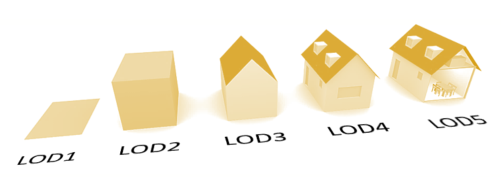
\includegraphics[width=0.65\linewidth]{images/LOD.png}
    \caption{Ejemplo de nivel de definición.}
\end{figure}

\subsubsection{Niveles de información}

Los niveles de información (LOI) definidos por la NBS-UK y descritos por el \citeA{bimforum2} se muestran a continuación:

\begin{itemize}
    \item \textbf{LOI 2 y 3:} el elemento modelado proporciona una descripción inicial para una entrega hacia el diseño.
    \item \textbf{LOI 4:} el elemento modelado proporciona una información suficiente para permitir la selección del producto de fabricante que cumpla con sus requerimientos. Esta información también puede ser utilizada para reemplazar un elemento durante el ciclo de vida del proyecto, una vez construido.
    \item \textbf{LOI 5:} el elemento modelado proporciona la información específica del producto de fabricante seleccionado o lo construido y entregado. Cualquier información adicional pertinente durante el proceso de construcción o instalación es indicada dentro de este nivel.
    \item \textbf{LOI 6:} el elemento modelado proporciona la información acumulada de los niveles anteriores y además considera información detallada del mantenimiento efectuado.
\end{itemize}

\subsubsection{Niveles de desarrollo}

Adicionalmente, el \textit{American Institute of Architects} (AIA) define al nivel de desarrollo como la forma de identificar requisitos mínimos y usos específicos a cada elemento del modelo, en un respectivo nivel. Los siguientes, son los niveles de desarrollo, en base a lo expuesto por el \citeA{bimforum2}:

\begin{itemize}
    \item \textbf{LOD 100:} el elemento puede ser representado gráficamente en el modelo con un símbolo u representación genérica. Estas representaciones muestran la existencia de un componente, pero no su forma, tamaño o ubicación precisa. La información debe ser considerada aproximada.
    \item \textbf{LOD 200:} el elemento se representa gráficamente como un sistema genérico de objeto, tamaño, forma, ubicación y orientación aproximados. La información no gráfica también es aproximada. Estas representaciones son respecto del volumen o espacio reservado.
    \item \textbf{LOD 300:} el elemento representa gráficamente como un objeto o sistema específico en términos de cantidad, tamaño, forma, ubicación y orientación. La información no gráfica se corresponde con la información gráfica. Las cantidades, dimensiones, formas, ubicación y orientación según lo diseñado se pueden obtener directamente a del elemento.
    \item \textbf{LOD 350:} igual al LOD 300, pero las representaciones se vinculan con otros elementos del modelo cercano o adjunto y se incluyen las partes tales como soportes o conexiones.
    \item \textbf{LOD 400:} LOD 350 más la modelación. Estas representaciones se modelan con la precisión y detalle suficiente para su fabricación e instalación.       
    \item \textbf{LOD 500:} el elemento modelado es una representación fiel del elemento de construcción ya ejecutado en obra, con su tamaño, forma, ubicación y orientación real en el proyecto. La información no gráfica está incluida en el objeto, así como sus vínculos con otros elementos. Estas representaciones se realizan una vez construido el proyecto y son las adecuadas para el mantenimiento y el funcionamiento del elemento en el inmueble.
\end{itemize}

\begin{figure}[H]
    \centering
    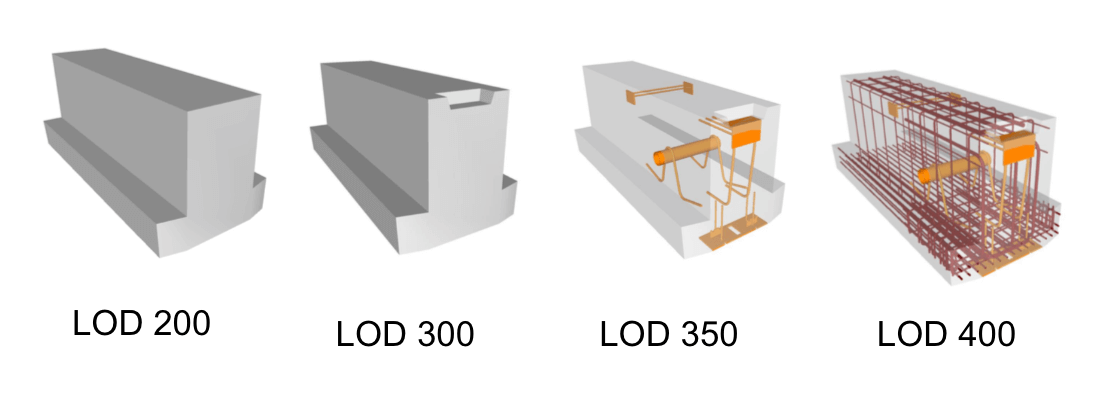
\includegraphics[width=0.95\linewidth]{images/lod-arch.jpg}
    \caption{Ejemplo de nivel de desarrollo.}
\end{figure}

\subsection{Madurez BIM} 

Existen diversos métodos y herramientas para estimar el nivel de madurez BIM de un proyecto. Por ejemplo, la NBIMS-USA\textregistered cuenta con un modelo de capacidades de madurez para definir la madurez de los modelos y permitir a los usuarios evaluar us prácticas y procesos basados en un espectro y funcionalidades técnicas definidas. El objetivo de las capacidades de madurez es proveer criterios de comparación y metas para el progreso en la madurez proyectos. Esta herramienta consiste de diez niveles de madurez, siendo diez el máximo \cite{trejo2018estudio}.

Por otro lado, la NBS-UK propone un modelo que consta de cuatro niveles, los que son \cite{trejo2018estudio}:


\begin{itemize}
    \item \textbf{Nivel 0:} no hay colaboración. CAD 2D solo utilizado en producción. Los \textit{outputs} son distribuidos en papel, en digital o una mezcla de ambos.
    \item \textbf{Nivel 1:} mezcla de CAD 3D para trabajo conceptual y 2D para documentación. Se administran estándares CAD y el intercambio electrónico de datos se lleva a cabo desde un entorno de datos común, a menudo administrado por el contratista. Los modelos no se comparten entre los miembros del equipo del proyecto.
    \item \textbf{Nivel 2:} trabajo colaborativo en que todas las partes usan sus propios modelos CAD en 3D, pero no necesariamente trabajan en un solo modelo compartido. La colaboración tiene que ver con la manera en que se intercambia la información entre las diferentes partes (formato de archivo común).
    \item \textbf{Nivel 3:} colaboración completa entre todas las disciplinas mediante el uso de un único modelo de proyecto compartido que se mantiene en un repositorio centralizado. Todas las partes pueden acceder y modificar ese mismo modelo y el beneficio es que elimina la capa final de riesgo de información conflictiva. Esto se conoce como ``Open BIM".
\end{itemize}

Para \citeA{succar2010building}, la madurez BIM se refiere a la mejora gradual y continua de la calidad, repetibilidad y predictibilidad dentro de una capacidad BIM disponible. La capacidad BIM, por su parte, hace referencia a las habilidades mínimas de una organización o equipo para entregar resultados medibles.

Así, pues, el índice de madurez BIM planteado por Succar consta de cinco niveles de madurez. Estos son: nivel incial, nivel definido, nivel gestionado, nivel integrado y nivel optimizado.

La Vicepresidencia de Proyectos de CODELCO, por su parte, utiliza la definición de Succar para asignar un \textit{rating} de madurez a sus proyectos. Para CODELCO, las cinco etapas definidas por Succar se han modificado someramente para ajustarse sus propias necesidades. Los niveles de madurez para CODELCO son, entonces, los que se detallan a continuación:

\begin{table}[H]
    \centering
    \caption{Niveles de madurez BIM de acuerdo a lo planteado por la Vicepresidencia de Proyectos, CODELCO.}
    \label{tab:niveles-madurez-codelco}
    \begin{tabular}{l p{0.65\linewidth}}
        \toprule
        \textbf{Niveles de madurez BIM} & \textbf{Descripción} \\
        \midrule
        \textbf{Nivel 0} & Nivel inicial pre BIM. Es un diseño a través de planos. \\
        \hline
        \textbf{Nivel 1} & Nivel definido. Consiste en un diseño a través de planos junto a un modelo 3D sin datos adicionales. \\
        \hline
        \textbf{Nivel 2} & Nivel gestionado. Modelo basado en la colaboración. Aquí el diseño es a través de un modelo 3D multidisciplinario con datos y gestión a través de planos. \\
        \hline
        \textbf{Nivel 3} & Nivel integrado. Existe una integración virtual 3D con datos entre distintos contratos de un proyecto, y la gestión a través de de un modelo 3D. \\
        \hline
        \textbf{Nivel 4} & Nivel optmizado. Post BIM. Consiste en un diseño virtual 3D con datos, multidisciplinario, colaborativo y con información integrada entre sistemas. \\
        \bottomrule
    \end{tabular}
\end{table}

Cabe mencionar, sin embargo, que las empresas e instituciones suelen desarrollar sus propios métodos para medir la madurez BIM.

\subsection{BIM en Chile}

El BIM en Chile comenzó su desarrollo desde el ámbito de la arquitectura, expandiéndose a ingeniería, construcción y operaciones. Los primeros indicios del uso de BIM se dieron en la infraestructura hospitalaria, dadas las exigencias en las licitaciones desde el 2009. Dados los beneficios obtenidos en estas experiencias, el BIM se hizo cada vez más atractivos para las demás áreas de la industria \cite{trejo2018estudio}.

El desarrollo de BIM en Chile ha sido monitoreado por distintas entidades, como lo son la CDT, el BIM Forum Chile, universidades, entre otros.

El \citeA{bimforum2}, según sus propias definiciones, es una instancia técnica y permanente, que convoca a los principales profesionales e instituciones relacionadas al BIM en Chile. Busca canalizar las inquietudes técnicas, el conocimiento y la información relacionados a BIM, constituyéndose también en una instancia de desarrollo, difusión y buenas prácticas para el desarrollo tecnológico en el sector construcción.

Los propósitos de BIM Forum Chile son netamente técnicos y sesiona bajo la coordinación de la Corporación de Desarrollo Tecnológico (CDT) de la Cámara Chilena de la Construcción (CChC). También es una instancia abierta y convocante, agrupando a las empresas y profesionales que puedan aportar sus conocimientos y experiencias al mejoramiento de las técnicas relacionadas a BIM.

\subsection{Ventajas de la metodología BIM}

En términos generales, la \citeA{lnb} indica que la principal ventaja es la visualización en 3D de lo que se está proyectando, permitiendo realizar ensayos o probar distintas configuraciones antes de la ejecución, cuantificación automática de cubicaciones, identificación de interferencias, fabricaciones e impulso en la industrialización de la construcción.

En esta línea, la \citeA{lnb} plantea las siguientes ventajas para los usuarios y para el proyecto:

\begin{itemize}
    \item El uso de la metodología y herramientas en general permite establecer un estándar de desarrollo de proyectos, un orden, una mejora de productividad; una vez superada la curva de aprendizaje, mayor rendimiento o menores plazos en el desarrollo de tareas habituales en los proyectos o abarcar más proyectos por la misma cantidad de profesionales, entre otras. El beneficio real que se obtenga de BIM depende de diversos factores, como los objetivos buscados por cada participante, la capacidad de comunicación entre actores, capacidades tecnológicas y humanas de cada oficina, entre otros.
    \item {El uso de BIM en general requiere de un mayor esfuerzo en la fase de diseño de los proyectos, pero esto se retribuye con la posibilidad de realizar ensayos, simulaciones virtuales y distintos tipos de análisis permitiendo la toma de mejores decisiones y más informadas. También se pueden observar menores inconsistencias e interferencias al momento de construir, sin mayores aumentos de plazos y con costos controlados, evitando las ineficiencias por falta de definiciones en el proyecto. Tener múltiples opciones de diseño sin la necesidad de modificar todo el universo de planos o documentación puesto que, al estar vinculadas, la actualización es automática.
    
    Si su uso durante todo el ciclo del proyecto es parte de los objetivos, los beneficios que puede llegar a generar en la planificación de las vías de acceso necesarias para el mantenimiento, en el rastreo y control de los componentes, en remodelaciones y posteriores demoliciones, pueden reflejar un ahorro final significativo en la totalidad de la vida del proyecto desde el punto de vista de la gestión de activos. Cabe destacar que el mayor ahorro de este nuevo proceso se produce en la fase de operación y mantenimiento.} 
\end{itemize}

Por otro lado, el \citeA{bimforum2} indica que:

\begin{quote}
    ``El mayor beneficio se encuentra cuando este modelo y la riqueza de información que incorpora, es usado en conjunto con aplicaciones de administración de edificios o Facilities Management (FM), sobre todo en proyectos complejos que requieren sistemas de apoyo para su funcionamiento como hospitales o industrias, para administrar las mantenciones y costos asociados a estos equipos."    
\end{quote}

Asimismo, la metodología BIM, considerada como plataforma de coordinación, puede tener dos efectos en el comportamiento de un contrato \cite{chang2014economic}: 

\begin{itemize}
    \item Digitalizar el diseño en un conjunto de objetos paramétricos 3D podría reducir la incidencia de malas interpretaciones de la información del diseño provenientes de errores humanos durante la transferencia de información. Digitalizar reduce, de manera inherente, la incidencia en las órdenes de cambio, lo que permite que el dueño del proyecto esté menos expuesto a retrasos en los pagos.
    \item El uso de la metodología BIM podría hacer posible que las empresas subcontratistas incorporasen sus inputs en el diseño digital durante una etapa temprana. Además, el uso de BIM facilita la detección de interferencias que podrían resultar en un cambio durante la etapa de construcción. Todo lo anterior también impacta en la reducción de la exposición a cambios indeseados del dueño.
\end{itemize}
